\section{Binary Search Trees}

\subsection{What is a binary search tree?}

\begin{description}
\descitem{12.1-1} \textit{For the set of $\{1, 4, 5, 10, 16, 17, 21\}$ of keys, draw binary search trees of heights $2$, $3$, $4$, $5$, and $6$.}

\begin{ex}
    \begin{figure}[H]
      \centering
      \begin{subfigure}[t]{.45\textwidth}
        \centering
        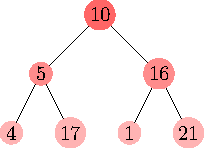
\includegraphics[scale=1]{img/12_1-1/12_1-1_1.pdf}
        \caption{$\text{hauteur} = 2 $}\label{fig:12_1-1_1}
      \end{subfigure}
      \begin{subfigure}[t]{.45\textwidth}
        \centering
        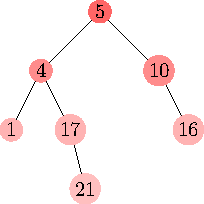
\includegraphics[scale=1]{img/12_1-1/12_1-1_2.pdf}
        \caption{$\text{hauteur} = 3 $}\label{fig:12_1-1_2}
      \end{subfigure}
      \begin{subfigure}[t]{.30\textwidth}
        \centering
        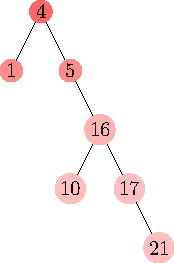
\includegraphics[scale=1]{img/12_1-1/12_1-1_3.pdf}
        \caption{$\text{hauteur} = 4 $}\label{fig:12_1-1_3}
      \end{subfigure}
      \begin{subfigure}[t]{.30\textwidth}
        \centering
        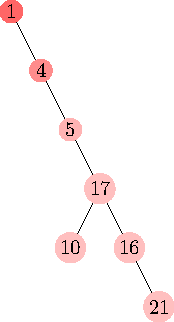
\includegraphics[scale=1]{img/12_1-1/12_1-1_4.pdf}
        \caption{$\text{hauteur} = 5 $}\label{fig:12_1-1_4}
      \end{subfigure}
      \begin{subfigure}[t]{.30\textwidth}
        \centering
        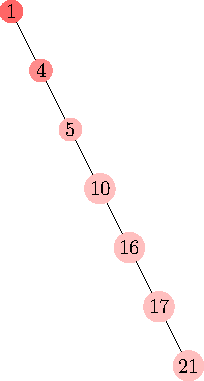
\includegraphics[scale=1]{img/12_1-1/12_1-1_5.pdf}
        \caption{$\text{hauteur} = 6 $}\label{fig:12_1-1_5}
      \end{subfigure}
      \caption{Exemples d'arbre binaire de recherche de hauteur respectivement $2, 3, 4, 5$ et $6$ remplit par l'ensemble $\{1, 4, 5, 10, 16, 17, 21\}$}
      \label{fig:binary-search-tree} 
    \end{figure}
\end{ex}
\descitem{12.1-2} \textit{What is the difference between the binary-search-tree property and the min-heap property (see page 153)? Can the min-heap property be used to print out the keys of an $n$-node tree in sorted order in $O(n)$ time? Show how, or explain why not.}

\begin{ex}
    Soient un nœud $n$, un nœud $l$ du sous-arbre gauche de $n$ et  un nœud $r$ du sous-arbre de droite de $n$. La propriété d'arbre binaire de recherche impose que $l \le n \le r$, alors que dans un tas-min, on ne peut seulement affirmer que $l \ge n$ et que $r \ge n$.

    Comme la relation entre $l$ et $r$ n'est pas connue dans un tas-min, on ne peut savoir dans quel sous-arbre apparait la prochaine clé en $O(n)$. Le tri par tas permet de faire cela en $O(n\lg n)$.  
\end{ex}

\end{description}
